\documentclass[1p]{elsarticle_modified}
%\bibliographystyle{elsarticle-num}

%\usepackage[colorlinks]{hyperref}
%\usepackage{abbrmath_seonhwa} %\Abb, \Ascr, \Acal ,\Abf, \Afrak
\usepackage{amsfonts}
\usepackage{amssymb}
\usepackage{amsmath}
\usepackage{amsthm}
\usepackage{scalefnt}
\usepackage{amsbsy}
\usepackage{kotex}
\usepackage{caption}
\usepackage{subfig}
\usepackage{color}
\usepackage{graphicx}
\usepackage{xcolor} %% white, black, red, green, blue, cyan, magenta, yellow
\usepackage{float}
\usepackage{setspace}
\usepackage{hyperref}

\usepackage{tikz}
\usetikzlibrary{arrows}

\usepackage{multirow}
\usepackage{array} % fixed length table
\usepackage{hhline}

%%%%%%%%%%%%%%%%%%%%%
\makeatletter
\renewcommand*\env@matrix[1][\arraystretch]{%
	\edef\arraystretch{#1}%
	\hskip -\arraycolsep
	\let\@ifnextchar\new@ifnextchar
	\array{*\c@MaxMatrixCols c}}
\makeatother %https://tex.stackexchange.com/questions/14071/how-can-i-increase-the-line-spacing-in-a-matrix
%%%%%%%%%%%%%%%

\usepackage[normalem]{ulem}

\newcommand{\msout}[1]{\ifmmode\text{\sout{\ensuremath{#1}}}\else\sout{#1}\fi}
%SOURCE: \msout is \stkout macro in https://tex.stackexchange.com/questions/20609/strikeout-in-math-mode

\newcommand{\cancel}[1]{
	\ifmmode
	{\color{red}\msout{#1}}
	\else
	{\color{red}\sout{#1}}
	\fi
}

\newcommand{\add}[1]{
	{\color{blue}\uwave{#1}}
}

\newcommand{\replace}[2]{
	\ifmmode
	{\color{red}\msout{#1}}{\color{blue}\uwave{#2}}
	\else
	{\color{red}\sout{#1}}{\color{blue}\uwave{#2}}
	\fi
}

\newcommand{\Sol}{\mathcal{S}} %segment
\newcommand{\D}{D} %diagram
\newcommand{\A}{\mathcal{A}} %arc


%%%%%%%%%%%%%%%%%%%%%%%%%%%%%5 test

\def\sl{\operatorname{\textup{SL}}(2,\Cbb)}
\def\psl{\operatorname{\textup{PSL}}(2,\Cbb)}
\def\quan{\mkern 1mu \triangleright \mkern 1mu}

\theoremstyle{definition}
\newtheorem{thm}{Theorem}[section]
\newtheorem{prop}[thm]{Proposition}
\newtheorem{lem}[thm]{Lemma}
\newtheorem{ques}[thm]{Question}
\newtheorem{cor}[thm]{Corollary}
\newtheorem{defn}[thm]{Definition}
\newtheorem{exam}[thm]{Example}
\newtheorem{rmk}[thm]{Remark}
\newtheorem{alg}[thm]{Algorithm}

\newcommand{\I}{\sqrt{-1}}
\begin{document}

%\begin{frontmatter}
%
%\title{Boundary parabolic representations of knots up to 8 crossings}
%
%%% Group authors per affiliation:
%\author{Yunhi Cho} 
%\address{Department of Mathematics, University of Seoul, Seoul, Korea}
%\ead{yhcho@uos.ac.kr}
%
%
%\author{Seonhwa Kim} %\fnref{s_kim}}
%\address{Center for Geometry and Physics, Institute for Basic Science, Pohang, 37673, Korea}
%\ead{ryeona17@ibs.re.kr}
%
%\author{Hyuk Kim}
%\address{Department of Mathematical Sciences, Seoul National University, Seoul 08826, Korea}
%\ead{hyukkim@snu.ac.kr}
%
%\author{Seokbeom Yoon}
%\address{Department of Mathematical Sciences, Seoul National University, Seoul, 08826,  Korea}
%\ead{sbyoon15@snu.ac.kr}
%
%\begin{abstract}
%We find all boundary parabolic representation of knots up to 8 crossings.
%
%\end{abstract}
%\begin{keyword}
%    \MSC[2010] 57M25 
%\end{keyword}
%
%\end{frontmatter}

%\linenumbers
%\tableofcontents
%
\newcommand\colored[1]{\textcolor{white}{\rule[-0.35ex]{0.8em}{1.4ex}}\kern-0.8em\color{red} #1}%
%\newcommand\colored[1]{\textcolor{white}{ #1}\kern-2.17ex	\textcolor{white}{ #1}\kern-1.81ex	\textcolor{white}{ #1}\kern-2.15ex\color{red}#1	}

{\Large $\underline{12a_{0507}~(K12a_{0507})}$}

\setlength{\tabcolsep}{10pt}
\renewcommand{\arraystretch}{1.6}
\vspace{1cm}\begin{tabular}{m{100pt}>{\centering\arraybackslash}m{274pt}}
\multirow{5}{120pt}{
	\centering
	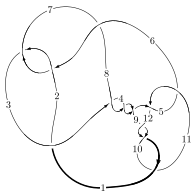
\includegraphics[width=112pt]{../../../GIT/diagram.site/Diagrams/png/1308_12a_0507.png}\\
\ \ \ A knot diagram\footnotemark}&
\allowdisplaybreaks
\textbf{Linearized knot diagam} \\
\cline{2-2}
 &
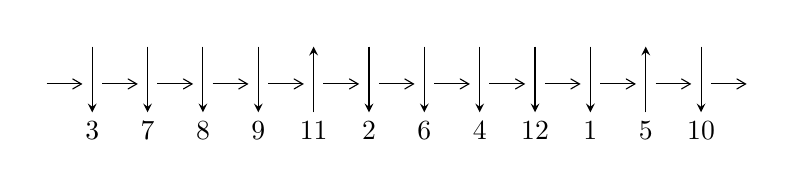
\begin{tikzpicture}[x=20pt, y=17pt]
	% nodes
	\node (C0) at (0, 0) {};
	\node (C1) at (1, 0) {};
	\node (C1U) at (1, +1) {};
	\node (C1D) at (1, -1) {3};

	\node (C2) at (2, 0) {};
	\node (C2U) at (2, +1) {};
	\node (C2D) at (2, -1) {7};

	\node (C3) at (3, 0) {};
	\node (C3U) at (3, +1) {};
	\node (C3D) at (3, -1) {8};

	\node (C4) at (4, 0) {};
	\node (C4U) at (4, +1) {};
	\node (C4D) at (4, -1) {9};

	\node (C5) at (5, 0) {};
	\node (C5U) at (5, +1) {};
	\node (C5D) at (5, -1) {11};

	\node (C6) at (6, 0) {};
	\node (C6U) at (6, +1) {};
	\node (C6D) at (6, -1) {2};

	\node (C7) at (7, 0) {};
	\node (C7U) at (7, +1) {};
	\node (C7D) at (7, -1) {6};

	\node (C8) at (8, 0) {};
	\node (C8U) at (8, +1) {};
	\node (C8D) at (8, -1) {4};

	\node (C9) at (9, 0) {};
	\node (C9U) at (9, +1) {};
	\node (C9D) at (9, -1) {12};

	\node (C10) at (10, 0) {};
	\node (C10U) at (10, +1) {};
	\node (C10D) at (10, -1) {1};

	\node (C11) at (11, 0) {};
	\node (C11U) at (11, +1) {};
	\node (C11D) at (11, -1) {5};

	\node (C12) at (12, 0) {};
	\node (C12U) at (12, +1) {};
	\node (C12D) at (12, -1) {10};
	\node (C13) at (13, 0) {};

	% arrows
	\draw[->,>={angle 60}]
	(C0) edge (C1) (C1) edge (C2) (C2) edge (C3) (C3) edge (C4) (C4) edge (C5) (C5) edge (C6) (C6) edge (C7) (C7) edge (C8) (C8) edge (C9) (C9) edge (C10) (C10) edge (C11) (C11) edge (C12) (C12) edge (C13) ;	\draw[->,>=stealth]
	(C1U) edge (C1D) (C2U) edge (C2D) (C3U) edge (C3D) (C4U) edge (C4D) (C5D) edge (C5U) (C6U) edge (C6D) (C7U) edge (C7D) (C8U) edge (C8D) (C9U) edge (C9D) (C10U) edge (C10D) (C11D) edge (C11U) (C12U) edge (C12D) ;
	\end{tikzpicture} \\
\hhline{~~} \\& 
\textbf{Solving Sequence} \\ \cline{2-2} 
 &
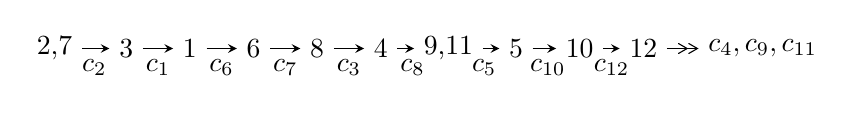
\begin{tikzpicture}[x=23pt, y=7pt]
	% node
	\node (A0) at (-1/8, 0) {2,7};
	\node (A1) at (1, 0) {3};
	\node (A2) at (2, 0) {1};
	\node (A3) at (3, 0) {6};
	\node (A4) at (4, 0) {8};
	\node (A5) at (5, 0) {4};
	\node (A6) at (97/16, 0) {9,11};
	\node (A7) at (57/8, 0) {5};
	\node (A8) at (65/8, 0) {10};
	\node (A9) at (73/8, 0) {12};
	\node (C1) at (1/2, -1) {$c_{2}$};
	\node (C2) at (3/2, -1) {$c_{1}$};
	\node (C3) at (5/2, -1) {$c_{6}$};
	\node (C4) at (7/2, -1) {$c_{7}$};
	\node (C5) at (9/2, -1) {$c_{3}$};
	\node (C6) at (11/2, -1) {$c_{8}$};
	\node (C7) at (53/8, -1) {$c_{5}$};
	\node (C8) at (61/8, -1) {$c_{10}$};
	\node (C9) at (69/8, -1) {$c_{12}$};
	\node (A10) at (11, 0) {$c_{4},c_{9},c_{11}$};

	% edge
	\draw[->,>=stealth]	
	(A0) edge (A1) (A1) edge (A2) (A2) edge (A3) (A3) edge (A4) (A4) edge (A5) (A5) edge (A6) (A6) edge (A7) (A7) edge (A8) (A8) edge (A9) ;
	\draw[->>,>={angle 60}]	
	(A9) edge (A10);
\end{tikzpicture} \\ 

\end{tabular} \\

\footnotetext{
The image of knot diagram is generated by the software ``\textbf{Draw programme}" developed by Andrew Bartholomew(\url{http://www.layer8.co.uk/maths/draw/index.htm\#Running-draw}), where we modified some parts for our purpose(\url{https://github.com/CATsTAILs/LinksPainter}).
}\phantom \\ \newline 
\centering \textbf{Ideals for irreducible components\footnotemark of $X_{\text{par}}$} 
 
\begin{align*}
I^u_{1}&=\langle 
u^{63}+u^{62}+\cdots+b+1,\;u^{64}+2 u^{63}+\cdots+a+2,\;u^{65}+2 u^{64}+\cdots+u+1\rangle \\
I^u_{2}&=\langle 
u^7- u^5+u^4+u^3+b+1,\;u^7- u^5+u^4+u^3+a+1,\;u^8- u^7- u^6+2 u^5+u^4-2 u^3+2 u-1\rangle \\
\\
\end{align*}
\raggedright * 2 irreducible components of $\dim_{\mathbb{C}}=0$, with total 73 representations.\\
\footnotetext{All coefficients of polynomials are rational numbers. But the coefficients are sometimes approximated in decimal forms when there is not enough margin.}
\newpage
\renewcommand{\arraystretch}{1}
\centering \section*{I. $I^u_{1}= \langle u^{63}+u^{62}+\cdots+b+1,\;u^{64}+2 u^{63}+\cdots+a+2,\;u^{65}+2 u^{64}+\cdots+u+1 \rangle$}
\flushleft \textbf{(i) Arc colorings}\\
\begin{tabular}{m{7pt} m{180pt} m{7pt} m{180pt} }
\flushright $a_{2}=$&$\begin{pmatrix}1\\0\end{pmatrix}$ \\
\flushright $a_{7}=$&$\begin{pmatrix}0\\u\end{pmatrix}$ \\
\flushright $a_{3}=$&$\begin{pmatrix}1\\u^2\end{pmatrix}$ \\
\flushright $a_{1}=$&$\begin{pmatrix}- u^2+1\\- u^4\end{pmatrix}$ \\
\flushright $a_{6}=$&$\begin{pmatrix}u\\u\end{pmatrix}$ \\
\flushright $a_{8}=$&$\begin{pmatrix}- u^3\\- u^3+u\end{pmatrix}$ \\
\flushright $a_{4}=$&$\begin{pmatrix}- u^8+u^6- u^4+1\\- u^8+2 u^6-2 u^4+2 u^2\end{pmatrix}$ \\
\flushright $a_{9}=$&$\begin{pmatrix}u^{13}-2 u^{11}+3 u^9-2 u^7- u\\u^{13}-3 u^{11}+5 u^9-6 u^7+4 u^5-3 u^3+u\end{pmatrix}$ \\
\flushright $a_{11}=$&$\begin{pmatrix}- u^{64}-2 u^{63}+\cdots+6 u-2\\- u^{63}- u^{62}+\cdots+2 u-1\end{pmatrix}$ \\
\flushright $a_{5}=$&$\begin{pmatrix}u^{18}-3 u^{16}+6 u^{14}-7 u^{12}+5 u^{10}-3 u^8- u^2+1\\u^{18}-4 u^{16}+9 u^{14}-14 u^{12}+15 u^{10}-14 u^8+10 u^6-6 u^4+3 u^2\end{pmatrix}$ \\
\flushright $a_{10}=$&$\begin{pmatrix}- u^{64}- u^{63}+\cdots+7 u-2\\- u^{64}- u^{63}+\cdots+u-1\end{pmatrix}$ \\
\flushright $a_{12}=$&$\begin{pmatrix}- u^{64}+11 u^{62}+\cdots+7 u-1\\-2 u^{64}- u^{63}+\cdots+u-1\end{pmatrix}$\\&\end{tabular}
\flushleft \textbf{(ii) Obstruction class $= -1$}\\~\\
\flushleft \textbf{(iii) Cusp Shapes $= 3 u^{64}+6 u^{63}+\cdots-13 u-3$}\\~\\
\newpage\renewcommand{\arraystretch}{1}
\flushleft \textbf{(iv) u-Polynomials at the component}\newline \\
\begin{tabular}{m{50pt}|m{274pt}}
Crossings & \hspace{64pt}u-Polynomials at each crossing \\
\hline $$\begin{aligned}c_{1},c_{7}\end{aligned}$$&$\begin{aligned}
&u^{65}+24 u^{64}+\cdots+17 u+1
\end{aligned}$\\
\hline $$\begin{aligned}c_{2},c_{6}\end{aligned}$$&$\begin{aligned}
&u^{65}-2 u^{64}+\cdots+u-1
\end{aligned}$\\
\hline $$\begin{aligned}c_{3},c_{4},c_{8}\end{aligned}$$&$\begin{aligned}
&u^{65}+2 u^{64}+\cdots+72 u-36
\end{aligned}$\\
\hline $$\begin{aligned}c_{5},c_{11}\end{aligned}$$&$\begin{aligned}
&u^{65}+u^{64}+\cdots+896 u+256
\end{aligned}$\\
\hline $$\begin{aligned}c_{9},c_{10},c_{12}\end{aligned}$$&$\begin{aligned}
&u^{65}-9 u^{64}+\cdots-9 u+1
\end{aligned}$\\
\hline
\end{tabular}\\~\\
\newpage\renewcommand{\arraystretch}{1}
\flushleft \textbf{(v) Riley Polynomials at the component}\newline \\
\begin{tabular}{m{50pt}|m{274pt}}
Crossings & \hspace{64pt}Riley Polynomials at each crossing \\
\hline $$\begin{aligned}c_{1},c_{7}\end{aligned}$$&$\begin{aligned}
&y^{65}+36 y^{64}+\cdots+41 y-1
\end{aligned}$\\
\hline $$\begin{aligned}c_{2},c_{6}\end{aligned}$$&$\begin{aligned}
&y^{65}-24 y^{64}+\cdots+17 y-1
\end{aligned}$\\
\hline $$\begin{aligned}c_{3},c_{4},c_{8}\end{aligned}$$&$\begin{aligned}
&y^{65}-72 y^{64}+\cdots+29736 y-1296
\end{aligned}$\\
\hline $$\begin{aligned}c_{5},c_{11}\end{aligned}$$&$\begin{aligned}
&y^{65}+51 y^{64}+\cdots+507904 y-65536
\end{aligned}$\\
\hline $$\begin{aligned}c_{9},c_{10},c_{12}\end{aligned}$$&$\begin{aligned}
&y^{65}-69 y^{64}+\cdots+49 y-1
\end{aligned}$\\
\hline
\end{tabular}\\~\\
\newpage\flushleft \textbf{(vi) Complex Volumes and Cusp Shapes}
$$\begin{array}{c|c|c}  
\text{Solutions to }I^u_{1}& \I (\text{vol} + \sqrt{-1}CS) & \text{Cusp shape}\\
 \hline 
\begin{aligned}
u &= \phantom{-}0.713224 + 0.687444 I \\
a &= -1.24609 - 1.61970 I \\
b &= -0.365613 - 1.272500 I\end{aligned}
 & \phantom{-}1.29911 + 1.50054 I & -6.43332 - 4.09954 I \\ \hline\begin{aligned}
u &= \phantom{-}0.713224 - 0.687444 I \\
a &= -1.24609 + 1.61970 I \\
b &= -0.365613 + 1.272500 I\end{aligned}
 & \phantom{-}1.29911 - 1.50054 I & -6.43332 + 4.09954 I \\ \hline\begin{aligned}
u &= -0.548659 + 0.822542 I \\
a &= \phantom{-}1.67765 - 1.87113 I \\
b &= \phantom{-}0.03464 - 1.54590 I\end{aligned}
 & -12.9972 - 8.8431 I & -12.85103 + 3.48991 I \\ \hline\begin{aligned}
u &= -0.548659 - 0.822542 I \\
a &= \phantom{-}1.67765 + 1.87113 I \\
b &= \phantom{-}0.03464 + 1.54590 I\end{aligned}
 & -12.9972 + 8.8431 I & -12.85103 - 3.48991 I \\ \hline\begin{aligned}
u &= \phantom{-}0.791470 + 0.591517 I \\
a &= \phantom{-}1.45052 + 0.22949 I \\
b &= \phantom{-}0.791445 - 0.191921 I\end{aligned}
 & -0.45144 - 1.99183 I & -13.03479 + 1.78533 I \\ \hline\begin{aligned}
u &= \phantom{-}0.791470 - 0.591517 I \\
a &= \phantom{-}1.45052 - 0.22949 I \\
b &= \phantom{-}0.791445 + 0.191921 I\end{aligned}
 & -0.45144 + 1.99183 I & -13.03479 - 1.78533 I \\ \hline\begin{aligned}
u &= -1.015680 + 0.168873 I \\
a &= \phantom{-}1.072100 + 0.272547 I \\
b &= \phantom{-}1.00409 - 1.15227 I\end{aligned}
 & -10.47320 + 4.58721 I & -18.5571 - 4.5138 I \\ \hline\begin{aligned}
u &= -1.015680 - 0.168873 I \\
a &= \phantom{-}1.072100 - 0.272547 I \\
b &= \phantom{-}1.00409 + 1.15227 I\end{aligned}
 & -10.47320 - 4.58721 I & -18.5571 + 4.5138 I \\ \hline\begin{aligned}
u &= \phantom{-}0.700275 + 0.763983 I \\
a &= \phantom{-}0.48960 + 2.63017 I \\
b &= -0.64142 + 2.04420 I\end{aligned}
 & -4.38452 + 4.13952 I & -11.02353 - 2.97070 I \\ \hline\begin{aligned}
u &= \phantom{-}0.700275 - 0.763983 I \\
a &= \phantom{-}0.48960 - 2.63017 I \\
b &= -0.64142 - 2.04420 I\end{aligned}
 & -4.38452 - 4.13952 I & -11.02353 + 2.97070 I\\
 \hline 
 \end{array}$$\newpage$$\begin{array}{c|c|c}  
\text{Solutions to }I^u_{1}& \I (\text{vol} + \sqrt{-1}CS) & \text{Cusp shape}\\
 \hline 
\begin{aligned}
u &= -0.533819 + 0.798870 I \\
a &= -1.46665 + 1.17530 I \\
b &= -0.159563 + 0.626147 I\end{aligned}
 & -5.93028 - 4.47135 I & -11.14289 + 3.00215 I \\ \hline\begin{aligned}
u &= -0.533819 - 0.798870 I \\
a &= -1.46665 - 1.17530 I \\
b &= -0.159563 - 0.626147 I\end{aligned}
 & -5.93028 + 4.47135 I & -11.14289 - 3.00215 I \\ \hline\begin{aligned}
u &= \phantom{-}0.518412 + 0.795387 I \\
a &= -1.70961 - 0.08232 I \\
b &= -0.94816 - 1.34212 I\end{aligned}
 & -8.23637 + 1.60432 I & -12.14095 - 0.18134 I \\ \hline\begin{aligned}
u &= \phantom{-}0.518412 - 0.795387 I \\
a &= -1.70961 + 0.08232 I \\
b &= -0.94816 + 1.34212 I\end{aligned}
 & -8.23637 - 1.60432 I & -12.14095 + 0.18134 I \\ \hline\begin{aligned}
u &= -0.812099 + 0.670235 I \\
a &= \phantom{-}1.52706 + 0.04285 I \\
b &= \phantom{-}1.43769 - 0.56681 I\end{aligned}
 & \phantom{-}2.51447 + 2.05945 I & \phantom{-0.000000 } 0. - 3.62781 I \\ \hline\begin{aligned}
u &= -0.812099 - 0.670235 I \\
a &= \phantom{-}1.52706 - 0.04285 I \\
b &= \phantom{-}1.43769 + 0.56681 I\end{aligned}
 & \phantom{-}2.51447 - 2.05945 I & \phantom{-0.000000 -}0. + 3.62781 I \\ \hline\begin{aligned}
u &= -0.705301 + 0.621394 I \\
a &= -1.92385 + 0.84589 I \\
b &= -1.55110 + 1.65367 I\end{aligned}
 & -1.222500 + 0.017209 I & -9.24300 - 1.12644 I \\ \hline\begin{aligned}
u &= -0.705301 - 0.621394 I \\
a &= -1.92385 - 0.84589 I \\
b &= -1.55110 - 1.65367 I\end{aligned}
 & -1.222500 - 0.017209 I & -9.24300 + 1.12644 I \\ \hline\begin{aligned}
u &= \phantom{-}0.937657\phantom{ +0.000000I} \\
a &= -1.59986\phantom{ +0.000000I} \\
b &= -0.575570\phantom{ +0.000000I}\end{aligned}
 & -5.51198\phantom{ +0.000000I} & -17.1080\phantom{ +0.000000I} \\ \hline\begin{aligned}
u &= -0.505383 + 0.783995 I \\
a &= \phantom{-}0.778262 - 0.689429 I \\
b &= -0.327984 + 0.239802 I\end{aligned}
 & -6.10999 + 1.30884 I & -11.57224 - 2.61156 I\\
 \hline 
 \end{array}$$\newpage$$\begin{array}{c|c|c}  
\text{Solutions to }I^u_{1}& \I (\text{vol} + \sqrt{-1}CS) & \text{Cusp shape}\\
 \hline 
\begin{aligned}
u &= -0.505383 - 0.783995 I \\
a &= \phantom{-}0.778262 + 0.689429 I \\
b &= -0.327984 - 0.239802 I\end{aligned}
 & -6.10999 - 1.30884 I & -11.57224 + 2.61156 I \\ \hline\begin{aligned}
u &= \phantom{-}0.552421 + 0.745317 I \\
a &= \phantom{-}0.802012 - 0.057028 I \\
b &= \phantom{-}0.441507 + 0.474951 I\end{aligned}
 & -1.66866 + 1.26457 I & -4.48163 - 0.64966 I \\ \hline\begin{aligned}
u &= \phantom{-}0.552421 - 0.745317 I \\
a &= \phantom{-}0.802012 + 0.057028 I \\
b &= \phantom{-}0.441507 - 0.474951 I\end{aligned}
 & -1.66866 - 1.26457 I & -4.48163 + 0.64966 I \\ \hline\begin{aligned}
u &= -0.921663 + 0.079540 I \\
a &= -0.505185 + 0.420325 I \\
b &= -0.43418 + 1.48058 I\end{aligned}
 & -3.61711 + 2.05218 I & -17.0578 - 5.0395 I \\ \hline\begin{aligned}
u &= -0.921663 - 0.079540 I \\
a &= -0.505185 - 0.420325 I \\
b &= -0.43418 - 1.48058 I\end{aligned}
 & -3.61711 - 2.05218 I & -17.0578 + 5.0395 I \\ \hline\begin{aligned}
u &= -0.467653 + 0.791706 I \\
a &= \phantom{-}0.021320 + 0.804749 I \\
b &= \phantom{-}1.170190 - 0.600782 I\end{aligned}
 & -13.4836 + 5.4777 I & -13.28643 - 3.27596 I \\ \hline\begin{aligned}
u &= -0.467653 - 0.791706 I \\
a &= \phantom{-}0.021320 - 0.804749 I \\
b &= \phantom{-}1.170190 + 0.600782 I\end{aligned}
 & -13.4836 - 5.4777 I & -13.28643 + 3.27596 I \\ \hline\begin{aligned}
u &= \phantom{-}0.984595 + 0.489919 I \\
a &= \phantom{-}0.486559 - 0.702071 I \\
b &= \phantom{-}1.188930 + 0.454218 I\end{aligned}
 & -8.70414 - 1.49648 I & \phantom{-0.000000 } 0 \\ \hline\begin{aligned}
u &= \phantom{-}0.984595 - 0.489919 I \\
a &= \phantom{-}0.486559 + 0.702071 I \\
b &= \phantom{-}1.188930 - 0.454218 I\end{aligned}
 & -8.70414 + 1.49648 I & \phantom{-0.000000 } 0 \\ \hline\begin{aligned}
u &= \phantom{-}0.923412 + 0.605274 I \\
a &= -0.457168 - 0.927717 I \\
b &= -0.76064 - 1.67724 I\end{aligned}
 & -0.89013 - 2.73765 I & \phantom{-0.000000 } 0\\
 \hline 
 \end{array}$$\newpage$$\begin{array}{c|c|c}  
\text{Solutions to }I^u_{1}& \I (\text{vol} + \sqrt{-1}CS) & \text{Cusp shape}\\
 \hline 
\begin{aligned}
u &= \phantom{-}0.923412 - 0.605274 I \\
a &= -0.457168 + 0.927717 I \\
b &= -0.76064 + 1.67724 I\end{aligned}
 & -0.89013 + 2.73765 I & \phantom{-0.000000 } 0 \\ \hline\begin{aligned}
u &= -0.888492 + 0.663349 I \\
a &= -0.41584 + 1.37057 I \\
b &= \phantom{-}0.137087 + 1.392720 I\end{aligned}
 & \phantom{-}2.27977 + 3.10358 I & \phantom{-0.000000 } 0 \\ \hline\begin{aligned}
u &= -0.888492 - 0.663349 I \\
a &= -0.41584 - 1.37057 I \\
b &= \phantom{-}0.137087 - 1.392720 I\end{aligned}
 & \phantom{-}2.27977 - 3.10358 I & \phantom{-0.000000 } 0 \\ \hline\begin{aligned}
u &= -1.11106\phantom{ +0.000000I} \\
a &= \phantom{-}0.266855\phantom{ +0.000000I} \\
b &= -0.278254\phantom{ +0.000000I}\end{aligned}
 & -7.21985\phantom{ +0.000000I} & -10.5080\phantom{ +0.000000I} \\ \hline\begin{aligned}
u &= -0.858807 + 0.738316 I \\
a &= -1.78012 - 2.04437 I \\
b &= -2.43706 - 1.24263 I\end{aligned}
 & -1.89391 + 2.79805 I & \phantom{-0.000000 } 0 \\ \hline\begin{aligned}
u &= -0.858807 - 0.738316 I \\
a &= -1.78012 + 2.04437 I \\
b &= -2.43706 + 1.24263 I\end{aligned}
 & -1.89391 - 2.79805 I & \phantom{-0.000000 } 0 \\ \hline\begin{aligned}
u &= \phantom{-}1.146070 + 0.010400 I \\
a &= -0.399146 - 0.884665 I \\
b &= -0.22151 - 2.08621 I\end{aligned}
 & -11.82220 - 2.96438 I & \phantom{-0.000000 } 0 \\ \hline\begin{aligned}
u &= \phantom{-}1.146070 - 0.010400 I \\
a &= -0.399146 + 0.884665 I \\
b &= -0.22151 + 2.08621 I\end{aligned}
 & -11.82220 + 2.96438 I & \phantom{-0.000000 } 0 \\ \hline\begin{aligned}
u &= -0.955422 + 0.633656 I \\
a &= \phantom{-}1.50663 - 1.77636 I \\
b &= \phantom{-}0.69599 - 1.98085 I\end{aligned}
 & -1.98303 + 4.94470 I & \phantom{-0.000000 } 0 \\ \hline\begin{aligned}
u &= -0.955422 - 0.633656 I \\
a &= \phantom{-}1.50663 + 1.77636 I \\
b &= \phantom{-}0.69599 + 1.98085 I\end{aligned}
 & -1.98303 - 4.94470 I & \phantom{-0.000000 } 0\\
 \hline 
 \end{array}$$\newpage$$\begin{array}{c|c|c}  
\text{Solutions to }I^u_{1}& \I (\text{vol} + \sqrt{-1}CS) & \text{Cusp shape}\\
 \hline 
\begin{aligned}
u &= -1.14899\phantom{ +0.000000I} \\
a &= -0.795555\phantom{ +0.000000I} \\
b &= \phantom{-}0.455262\phantom{ +0.000000I}\end{aligned}
 & -14.0593\phantom{ +0.000000I} & -18.0700\phantom{ +0.000000I} \\ \hline\begin{aligned}
u &= \phantom{-}1.156610 + 0.029881 I \\
a &= \phantom{-}0.959308 + 0.424441 I \\
b &= \phantom{-}0.45584 + 1.79793 I\end{aligned}
 & -19.1194 - 7.3744 I & \phantom{-0.000000 } 0 \\ \hline\begin{aligned}
u &= \phantom{-}1.156610 - 0.029881 I \\
a &= \phantom{-}0.959308 - 0.424441 I \\
b &= \phantom{-}0.45584 - 1.79793 I\end{aligned}
 & -19.1194 + 7.3744 I & \phantom{-0.000000 } 0 \\ \hline\begin{aligned}
u &= \phantom{-}0.956552 + 0.664807 I \\
a &= \phantom{-}1.79937 + 0.87406 I \\
b &= \phantom{-}1.97712 + 1.72485 I\end{aligned}
 & \phantom{-}0.56939 - 6.73062 I & \phantom{-0.000000 } 0 \\ \hline\begin{aligned}
u &= \phantom{-}0.956552 - 0.664807 I \\
a &= \phantom{-}1.79937 - 0.87406 I \\
b &= \phantom{-}1.97712 - 1.72485 I\end{aligned}
 & \phantom{-}0.56939 + 6.73062 I & \phantom{-0.000000 } 0 \\ \hline\begin{aligned}
u &= \phantom{-}0.981422 + 0.702007 I \\
a &= -2.70793 - 0.03543 I \\
b &= -3.06189 - 1.09293 I\end{aligned}
 & -5.22876 - 9.69725 I & \phantom{-0.000000 } 0 \\ \hline\begin{aligned}
u &= \phantom{-}0.981422 - 0.702007 I \\
a &= -2.70793 + 0.03543 I \\
b &= -3.06189 + 1.09293 I\end{aligned}
 & -5.22876 + 9.69725 I & \phantom{-0.000000 } 0 \\ \hline\begin{aligned}
u &= \phantom{-}1.040310 + 0.653623 I \\
a &= -0.290402 - 0.811750 I \\
b &= \phantom{-}0.140732 - 1.060590 I\end{aligned}
 & -3.08664 - 6.59798 I & \phantom{-0.000000 } 0 \\ \hline\begin{aligned}
u &= \phantom{-}1.040310 - 0.653623 I \\
a &= -0.290402 + 0.811750 I \\
b &= \phantom{-}0.140732 + 1.060590 I\end{aligned}
 & -3.08664 + 6.59798 I & \phantom{-0.000000 } 0 \\ \hline\begin{aligned}
u &= -1.064460 + 0.646027 I \\
a &= -0.450969 + 0.418508 I \\
b &= -1.12284 + 1.29370 I\end{aligned}
 & -7.74953 + 4.07259 I & \phantom{-0.000000 } 0\\
 \hline 
 \end{array}$$\newpage$$\begin{array}{c|c|c}  
\text{Solutions to }I^u_{1}& \I (\text{vol} + \sqrt{-1}CS) & \text{Cusp shape}\\
 \hline 
\begin{aligned}
u &= -1.064460 - 0.646027 I \\
a &= -0.450969 - 0.418508 I \\
b &= -1.12284 - 1.29370 I\end{aligned}
 & -7.74953 - 4.07259 I & \phantom{-0.000000 } 0 \\ \hline\begin{aligned}
u &= -1.074890 + 0.630986 I \\
a &= \phantom{-}0.307606 + 0.701773 I \\
b &= \phantom{-}1.351880 - 0.171332 I\end{aligned}
 & -15.2686 - 0.1519 I & \phantom{-0.000000 } 0 \\ \hline\begin{aligned}
u &= -1.074890 - 0.630986 I \\
a &= \phantom{-}0.307606 - 0.701773 I \\
b &= \phantom{-}1.351880 + 0.171332 I\end{aligned}
 & -15.2686 + 0.1519 I & \phantom{-0.000000 } 0 \\ \hline\begin{aligned}
u &= \phantom{-}1.066140 + 0.653704 I \\
a &= \phantom{-}0.82798 + 1.79881 I \\
b &= -0.17076 + 2.34794 I\end{aligned}
 & -9.85329 - 7.04987 I & \phantom{-0.000000 } 0 \\ \hline\begin{aligned}
u &= \phantom{-}1.066140 - 0.653704 I \\
a &= \phantom{-}0.82798 - 1.79881 I \\
b &= -0.17076 - 2.34794 I\end{aligned}
 & -9.85329 + 7.04987 I & \phantom{-0.000000 } 0 \\ \hline\begin{aligned}
u &= -1.063690 + 0.660571 I \\
a &= \phantom{-}1.27520 - 1.15879 I \\
b &= \phantom{-}1.66073 - 2.19821 I\end{aligned}
 & -7.49945 + 9.95718 I & \phantom{-0.000000 } 0 \\ \hline\begin{aligned}
u &= -1.063690 - 0.660571 I \\
a &= \phantom{-}1.27520 + 1.15879 I \\
b &= \phantom{-}1.66073 + 2.19821 I\end{aligned}
 & -7.49945 - 9.95718 I & \phantom{-0.000000 } 0 \\ \hline\begin{aligned}
u &= -1.068690 + 0.673015 I \\
a &= -2.21159 + 1.26271 I \\
b &= -2.42067 + 2.56720 I\end{aligned}
 & -14.5530 + 14.4409 I & \phantom{-0.000000 } 0 \\ \hline\begin{aligned}
u &= -1.068690 - 0.673015 I \\
a &= -2.21159 - 1.26271 I \\
b &= -2.42067 - 2.56720 I\end{aligned}
 & -14.5530 - 14.4409 I & \phantom{-0.000000 } 0 \\ \hline\begin{aligned}
u &= \phantom{-}0.683701\phantom{ +0.000000I} \\
a &= \phantom{-}0.602547\phantom{ +0.000000I} \\
b &= \phantom{-}0.0385752\phantom{ +0.000000I}\end{aligned}
 & -1.02307\phantom{ +0.000000I} & -9.31980\phantom{ +0.000000I}\\
 \hline 
 \end{array}$$\newpage$$\begin{array}{c|c|c}  
\text{Solutions to }I^u_{1}& \I (\text{vol} + \sqrt{-1}CS) & \text{Cusp shape}\\
 \hline 
\begin{aligned}
u &= \phantom{-}0.211468 + 0.588502 I \\
a &= -0.736413 - 0.786410 I \\
b &= \phantom{-}1.212590 + 0.233332 I\end{aligned}
 & -6.70249 - 2.38114 I & -11.80434 + 2.89982 I \\ \hline\begin{aligned}
u &= \phantom{-}0.211468 - 0.588502 I \\
a &= -0.736413 + 0.786410 I \\
b &= \phantom{-}1.212590 - 0.233332 I\end{aligned}
 & -6.70249 + 2.38114 I & -11.80434 - 2.89982 I \\ \hline\begin{aligned}
u &= \phantom{-}0.212478 + 0.317081 I \\
a &= \phantom{-}0.920282 + 1.026800 I \\
b &= -0.309776 - 0.311699 I\end{aligned}
 & -0.431525 - 0.957888 I & -7.32117 + 6.97948 I \\ \hline\begin{aligned}
u &= \phantom{-}0.212478 - 0.317081 I \\
a &= \phantom{-}0.920282 - 1.026800 I \\
b &= -0.309776 + 0.311699 I\end{aligned}
 & -0.431525 + 0.957888 I & -7.32117 - 6.97948 I \\ \hline\begin{aligned}
u &= -0.301622\phantom{ +0.000000I} \\
a &= -2.67493\phantom{ +0.000000I} \\
b &= -1.17462\phantom{ +0.000000I}\end{aligned}
 & -2.05866\phantom{ +0.000000I} & -0.865930\phantom{ +0.000000I}\\
 \hline 
 \end{array}$$\newpage\newpage\renewcommand{\arraystretch}{1}
\centering \section*{II. $I^u_{2}= \langle u^7- u^5+u^4+u^3+b+1,\;u^7- u^5+u^4+u^3+a+1,\;u^8- u^7- u^6+2 u^5+u^4-2 u^3+2 u-1 \rangle$}
\flushleft \textbf{(i) Arc colorings}\\
\begin{tabular}{m{7pt} m{180pt} m{7pt} m{180pt} }
\flushright $a_{2}=$&$\begin{pmatrix}1\\0\end{pmatrix}$ \\
\flushright $a_{7}=$&$\begin{pmatrix}0\\u\end{pmatrix}$ \\
\flushright $a_{3}=$&$\begin{pmatrix}1\\u^2\end{pmatrix}$ \\
\flushright $a_{1}=$&$\begin{pmatrix}- u^2+1\\- u^4\end{pmatrix}$ \\
\flushright $a_{6}=$&$\begin{pmatrix}u\\u\end{pmatrix}$ \\
\flushright $a_{8}=$&$\begin{pmatrix}- u^3\\- u^3+u\end{pmatrix}$ \\
\flushright $a_{4}=$&$\begin{pmatrix}- u^7+2 u^5-2 u^3+2 u\\- u^7+u^6+2 u^5- u^4-2 u^3+2 u^2+2 u-1\end{pmatrix}$ \\
\flushright $a_{9}=$&$\begin{pmatrix}u^2-1\\u^4\end{pmatrix}$ \\
\flushright $a_{11}=$&$\begin{pmatrix}- u^7+u^5- u^4- u^3-1\\- u^7+u^5- u^4- u^3-1\end{pmatrix}$ \\
\flushright $a_{5}=$&$\begin{pmatrix}u\\u\end{pmatrix}$ \\
\flushright $a_{10}=$&$\begin{pmatrix}- u^7+u^5- u^4- u^3+u^2-2\\- u^7+u^5- u^3-1\end{pmatrix}$ \\
\flushright $a_{12}=$&$\begin{pmatrix}- u^7+u^5- u^4- u^3-1\\- u^7+u^5- u^4- u^3-1\end{pmatrix}$\\&\end{tabular}
\flushleft \textbf{(ii) Obstruction class $= 1$}\\~\\
\flushleft \textbf{(iii) Cusp Shapes $= -6 u^7+u^6+11 u^5-8 u^4-11 u^3+7 u^2+4 u-23$}\\~\\
\newpage\renewcommand{\arraystretch}{1}
\flushleft \textbf{(iv) u-Polynomials at the component}\newline \\
\begin{tabular}{m{50pt}|m{274pt}}
Crossings & \hspace{64pt}u-Polynomials at each crossing \\
\hline $$\begin{aligned}c_{1}\end{aligned}$$&$\begin{aligned}
&u^8-3 u^7+7 u^6-10 u^5+11 u^4-10 u^3+6 u^2-4 u+1
\end{aligned}$\\
\hline $$\begin{aligned}c_{2}\end{aligned}$$&$\begin{aligned}
&u^8- u^7- u^6+2 u^5+u^4-2 u^3+2 u-1
\end{aligned}$\\
\hline $$\begin{aligned}c_{3},c_{4}\end{aligned}$$&$\begin{aligned}
&u^8+u^7-3 u^6-2 u^5+3 u^4+2 u-1
\end{aligned}$\\
\hline $$\begin{aligned}c_{5},c_{11}\end{aligned}$$&$\begin{aligned}
&u^8
\end{aligned}$\\
\hline $$\begin{aligned}c_{6}\end{aligned}$$&$\begin{aligned}
&u^8+u^7- u^6-2 u^5+u^4+2 u^3-2 u-1
\end{aligned}$\\
\hline $$\begin{aligned}c_{7}\end{aligned}$$&$\begin{aligned}
&u^8+3 u^7+7 u^6+10 u^5+11 u^4+10 u^3+6 u^2+4 u+1
\end{aligned}$\\
\hline $$\begin{aligned}c_{8}\end{aligned}$$&$\begin{aligned}
&u^8- u^7-3 u^6+2 u^5+3 u^4-2 u-1
\end{aligned}$\\
\hline $$\begin{aligned}c_{9},c_{10}\end{aligned}$$&$\begin{aligned}
&(u-1)^8
\end{aligned}$\\
\hline $$\begin{aligned}c_{12}\end{aligned}$$&$\begin{aligned}
&(u+1)^8
\end{aligned}$\\
\hline
\end{tabular}\\~\\
\newpage\renewcommand{\arraystretch}{1}
\flushleft \textbf{(v) Riley Polynomials at the component}\newline \\
\begin{tabular}{m{50pt}|m{274pt}}
Crossings & \hspace{64pt}Riley Polynomials at each crossing \\
\hline $$\begin{aligned}c_{1},c_{7}\end{aligned}$$&$\begin{aligned}
&y^8+5 y^7+11 y^6+6 y^5-17 y^4-34 y^3-22 y^2-4 y+1
\end{aligned}$\\
\hline $$\begin{aligned}c_{2},c_{6}\end{aligned}$$&$\begin{aligned}
&y^8-3 y^7+7 y^6-10 y^5+11 y^4-10 y^3+6 y^2-4 y+1
\end{aligned}$\\
\hline $$\begin{aligned}c_{3},c_{4},c_{8}\end{aligned}$$&$\begin{aligned}
&y^8-7 y^7+19 y^6-22 y^5+3 y^4+14 y^3-6 y^2-4 y+1
\end{aligned}$\\
\hline $$\begin{aligned}c_{5},c_{11}\end{aligned}$$&$\begin{aligned}
&y^8
\end{aligned}$\\
\hline $$\begin{aligned}c_{9},c_{10},c_{12}\end{aligned}$$&$\begin{aligned}
&(y-1)^8
\end{aligned}$\\
\hline
\end{tabular}\\~\\
\newpage\flushleft \textbf{(vi) Complex Volumes and Cusp Shapes}
$$\begin{array}{c|c|c}  
\text{Solutions to }I^u_{2}& \I (\text{vol} + \sqrt{-1}CS) & \text{Cusp shape}\\
 \hline 
\begin{aligned}
u &= \phantom{-}0.570868 + 0.730671 I \\
a &= -0.325934 - 0.693334 I \\
b &= -0.325934 - 0.693334 I\end{aligned}
 & -2.68559 + 1.13123 I & -13.35119 - 0.17229 I \\ \hline\begin{aligned}
u &= \phantom{-}0.570868 - 0.730671 I \\
a &= -0.325934 + 0.693334 I \\
b &= -0.325934 + 0.693334 I\end{aligned}
 & -2.68559 - 1.13123 I & -13.35119 + 0.17229 I \\ \hline\begin{aligned}
u &= -0.855237 + 0.665892 I \\
a &= \phantom{-}1.03462 + 0.99451 I \\
b &= \phantom{-}1.03462 + 0.99451 I\end{aligned}
 & \phantom{-}0.51448 + 2.57849 I & -6.04880 - 3.90294 I \\ \hline\begin{aligned}
u &= -0.855237 - 0.665892 I \\
a &= \phantom{-}1.03462 - 0.99451 I \\
b &= \phantom{-}1.03462 - 0.99451 I\end{aligned}
 & \phantom{-}0.51448 - 2.57849 I & -6.04880 + 3.90294 I \\ \hline\begin{aligned}
u &= -1.09818\phantom{ +0.000000I} \\
a &= -0.801005\phantom{ +0.000000I} \\
b &= -0.801005\phantom{ +0.000000I}\end{aligned}
 & -8.14766\phantom{ +0.000000I} & -20.2760\phantom{ +0.000000I} \\ \hline\begin{aligned}
u &= \phantom{-}1.031810 + 0.655470 I \\
a &= \phantom{-}0.842429 + 0.289836 I \\
b &= \phantom{-}0.842429 + 0.289836 I\end{aligned}
 & -4.02461 - 6.44354 I & -15.5815 + 4.6831 I \\ \hline\begin{aligned}
u &= \phantom{-}1.031810 - 0.655470 I \\
a &= \phantom{-}0.842429 - 0.289836 I \\
b &= \phantom{-}0.842429 - 0.289836 I\end{aligned}
 & -4.02461 + 6.44354 I & -15.5815 - 4.6831 I \\ \hline\begin{aligned}
u &= \phantom{-}0.603304\phantom{ +0.000000I} \\
a &= -1.30123\phantom{ +0.000000I} \\
b &= -1.30123\phantom{ +0.000000I}\end{aligned}
 & -2.48997\phantom{ +0.000000I} & -20.7610\phantom{ +0.000000I}\\
 \hline 
 \end{array}$$\newpage
\newpage\renewcommand{\arraystretch}{1}
\centering \section*{ III. u-Polynomials}
\begin{tabular}{m{50pt}|m{274pt}}
Crossings & \hspace{64pt}u-Polynomials at each crossing \\
\hline $$\begin{aligned}c_{1}\end{aligned}$$&$\begin{aligned}
&(u^8-3 u^7+7 u^6-10 u^5+11 u^4-10 u^3+6 u^2-4 u+1)\\
&\cdot(u^{65}+24 u^{64}+\cdots+17 u+1)
\end{aligned}$\\
\hline $$\begin{aligned}c_{2}\end{aligned}$$&$\begin{aligned}
&(u^8- u^7+\cdots+2 u-1)(u^{65}-2 u^{64}+\cdots+u-1)
\end{aligned}$\\
\hline $$\begin{aligned}c_{3},c_{4}\end{aligned}$$&$\begin{aligned}
&(u^8+u^7-3 u^6-2 u^5+3 u^4+2 u-1)(u^{65}+2 u^{64}+\cdots+72 u-36)
\end{aligned}$\\
\hline $$\begin{aligned}c_{5},c_{11}\end{aligned}$$&$\begin{aligned}
&u^8(u^{65}+u^{64}+\cdots+896 u+256)
\end{aligned}$\\
\hline $$\begin{aligned}c_{6}\end{aligned}$$&$\begin{aligned}
&(u^8+u^7+\cdots-2 u-1)(u^{65}-2 u^{64}+\cdots+u-1)
\end{aligned}$\\
\hline $$\begin{aligned}c_{7}\end{aligned}$$&$\begin{aligned}
&(u^8+3 u^7+7 u^6+10 u^5+11 u^4+10 u^3+6 u^2+4 u+1)\\
&\cdot(u^{65}+24 u^{64}+\cdots+17 u+1)
\end{aligned}$\\
\hline $$\begin{aligned}c_{8}\end{aligned}$$&$\begin{aligned}
&(u^8- u^7-3 u^6+2 u^5+3 u^4-2 u-1)(u^{65}+2 u^{64}+\cdots+72 u-36)
\end{aligned}$\\
\hline $$\begin{aligned}c_{9},c_{10}\end{aligned}$$&$\begin{aligned}
&((u-1)^8)(u^{65}-9 u^{64}+\cdots-9 u+1)
\end{aligned}$\\
\hline $$\begin{aligned}c_{12}\end{aligned}$$&$\begin{aligned}
&((u+1)^8)(u^{65}-9 u^{64}+\cdots-9 u+1)
\end{aligned}$\\
\hline
\end{tabular}\newpage\renewcommand{\arraystretch}{1}
\centering \section*{ IV. Riley Polynomials}
\begin{tabular}{m{50pt}|m{274pt}}
Crossings & \hspace{64pt}Riley Polynomials at each crossing \\
\hline $$\begin{aligned}c_{1},c_{7}\end{aligned}$$&$\begin{aligned}
&(y^8+5 y^7+11 y^6+6 y^5-17 y^4-34 y^3-22 y^2-4 y+1)\\
&\cdot(y^{65}+36 y^{64}+\cdots+41 y-1)
\end{aligned}$\\
\hline $$\begin{aligned}c_{2},c_{6}\end{aligned}$$&$\begin{aligned}
&(y^8-3 y^7+7 y^6-10 y^5+11 y^4-10 y^3+6 y^2-4 y+1)\\
&\cdot(y^{65}-24 y^{64}+\cdots+17 y-1)
\end{aligned}$\\
\hline $$\begin{aligned}c_{3},c_{4},c_{8}\end{aligned}$$&$\begin{aligned}
&(y^8-7 y^7+19 y^6-22 y^5+3 y^4+14 y^3-6 y^2-4 y+1)\\
&\cdot(y^{65}-72 y^{64}+\cdots+29736 y-1296)
\end{aligned}$\\
\hline $$\begin{aligned}c_{5},c_{11}\end{aligned}$$&$\begin{aligned}
&y^8(y^{65}+51 y^{64}+\cdots+507904 y-65536)
\end{aligned}$\\
\hline $$\begin{aligned}c_{9},c_{10},c_{12}\end{aligned}$$&$\begin{aligned}
&((y-1)^8)(y^{65}-69 y^{64}+\cdots+49 y-1)
\end{aligned}$\\
\hline
\end{tabular}
\vskip 2pc
\end{document}